%\documentclass[]{article}
\documentclass[11pt]{article}
\usepackage[usenames,dvipsnames]{xcolor}

\usepackage[T1]{fontenc}
%\usepackage{lmodern}
\usepackage{tgtermes}
\usepackage{amssymb,amsmath}
%\usepackage[margin=1in]{geometry}
\usepackage[letterpaper,bottom=1in,top=1in,right=1.25in,left=1.25in,includemp=FALSE]{geometry}
\usepackage{pdfpages}
\usepackage[small]{caption}

\usepackage{ifxetex,ifluatex}
\usepackage{fixltx2e} % provides \textsubscript
% use microtype if available
\IfFileExists{microtype.sty}{\usepackage{microtype}}{}
\ifnum 0\ifxetex 1\fi\ifluatex 1\fi=0 % if pdftex
\usepackage[utf8]{inputenc}
\else % if luatex or xelatex
\usepackage{fontspec}
\ifxetex
\usepackage{xltxtra,xunicode}
\fi
\defaultfontfeatures{Mapping=tex-text,Scale=MatchLowercase}
\newcommand{\euro}{€}
\fi
%

\usepackage{fancyvrb}

\usepackage{ctable,longtable}

\usepackage[section]{placeins}
\usepackage{float} % provides the H option for float placement
\restylefloat{figure}
\usepackage{dcolumn} % allows for different column alignments
\newcolumntype{.}{D{.}{.}{1.2}}

\usepackage{booktabs} % nicer horizontal rules in tables

%Assume we want graphics always
\usepackage{graphicx}
% We will generate all images so they have a width \maxwidth. This means
% that they will get their normal width if they fit onto the page, but
% are scaled down if they would overflow the margins.
%% \makeatletter
%% \def\maxwidth{\ifdim\Gin@nat@width>\linewidth\linewidth
%%   \else\Gin@nat@width\fi}
%% \makeatother
%% \let\Oldincludegraphics\includegraphics
%% \renewcommand{\includegraphics}[1]{\Oldincludegraphics[width=\maxwidth]{#1}}
\graphicspath{{.}{../Soccom_Code/socom_2013/}}


%% \ifxetex
%% \usepackage[pagebackref=true, setpagesize=false, % page size defined by xetex
%% unicode=false, % unicode breaks when used with xetex
%% xetex]{hyperref}
%% \else
\usepackage[pagebackref=true, unicode=true, bookmarks=true, pdftex]{hyperref}
% \fi


\hypersetup{breaklinks=true,
  bookmarks=true,
  pdfauthor={Christopher Grady, Rebecca Wolfe, Danjuma Dawop, and Lisa Inks},
  pdftitle={Promoting Peace Amidst Group Conflict: An Intergroup Contact Field Experiment in Nigeria},
  colorlinks=true,
  linkcolor=BrickRed,
  citecolor=blue, %MidnightBlue,
  urlcolor=BrickRed,
  % urlcolor=blue,
  % linkcolor=magenta,
  pdfborder={0 0 0}}

%\setlength{\parindent}{0pt}
%\setlength{\parskip}{6pt plus 2pt minus 1pt}
\usepackage{parskip}
\setlength{\emergencystretch}{3em}  % prevent overfull lines
\providecommand{\tightlist}{%
  \setlength{\itemsep}{0pt}\setlength{\parskip}{0pt}}

%% Insist on this.
\setcounter{secnumdepth}{2}

\VerbatimFootnotes % allows verbatim text in footnotes

\title{Promoting Peace Amidst Group Conflict: An Intergroup Contact Field
Experiment in Nigeria}

\author{
Christopher Grady, Rebecca Wolfe, Danjuma Dawop, and Lisa Inks
}


\date{May 31, 2019}


\usepackage{versions}
\makeatletter
\renewcommand*\versionmessage[2]{\typeout{*** `#1' #2. ***}}
\renewcommand*\beginmarkversion{\sffamily}
  \renewcommand*\endmarkversion{}
\makeatother

\excludeversion{comment}

%\usepackage[margins=1in]{geometry}

\usepackage[compact,bottomtitles]{titlesec}
%\titleformat{ ⟨command⟩}[⟨shape⟩]{⟨format⟩}{⟨label⟩}{⟨sep⟩}{⟨before⟩}[⟨after⟩]
\titleformat{\section}[hang]{\Large\bfseries}{\thesection}{.5em}{\hspace{0in}}[\vspace{-.2\baselineskip}]
\titleformat{\subsection}[hang]{\large\bfseries}{\thesubsection}{.5em}{\hspace{0in}}[\vspace{-.2\baselineskip}]
%\titleformat{\subsubsection}[hang]{\bfseries}{\thesubsubsection}{.5em}{\hspace{0in}}[\vspace{-.2\baselineskip}]
\titleformat{\subsubsection}[hang]{\bfseries}{\thesubsubsection}{1ex}{\hspace{0in}}[\vspace{-.2\baselineskip}]
\titleformat{\paragraph}[runin]{\bfseries\itshape}{\theparagraph}{1ex}{}{\vspace{-.2\baselineskip}}
%\titleformat{\paragraph}[runin]{\itshape}{\theparagraph}{1ex}{}{\vspace{-.2\baselineskip}}

%%\titleformat{\subsection}[hang]{\bfseries}{\thesubsection}{.5em}{\hspace{0in}}[\vspace{-.2\baselineskip}]
%%%\titleformat*{\subsection}{\bfseries\scshape}
%%%\titleformat{\subsubsection}[leftmargin]{\footnotesize\filleft}{\thesubsubsection}{.5em}{}{}
%%\titleformat{\subsubsection}[hang]{\small\bfseries}{\thesubsubsection}{.5em}{\hspace{0in}}[\vspace{-.2\baselineskip}]
%%\titleformat{\paragraph}[runin]{\itshape}{\theparagraph}{1ex}{}{\vspace{-.5\baselineskip}}

%\titlespacing*{ ⟨command⟩}{⟨left⟩}{⟨beforesep⟩}{⟨aftersep⟩}[⟨right⟩]
\titlespacing{\section}{0pc}{1.5ex plus .1ex minus .2ex}{.5ex plus .1ex minus .1ex}
\titlespacing{\subsection}{0pc}{1.5ex plus .1ex minus .2ex}{.5ex plus .1ex minus .1ex}
\titlespacing{\subsubsection}{0pc}{1.5ex plus .1ex minus .2ex}{.5ex plus .1ex minus .1ex}



%% These next lines tell latex that it is ok to have a single graphic
%% taking up most of a page, and they also decrease the space around
%% figures and tables.
\renewcommand\floatpagefraction{.9}
\renewcommand\topfraction{.9}
\renewcommand\bottomfraction{.9}
\renewcommand\textfraction{.1}
\setcounter{totalnumber}{50}
\setcounter{topnumber}{50}
\setcounter{bottomnumber}{50}
\setlength{\intextsep}{2ex}
\setlength{\floatsep}{2ex}
\setlength{\textfloatsep}{2ex}



\begin{document}
\VerbatimFootnotes

%\begin{titlepage}
%  \maketitle
%\vspace{2in}
%
%\begin{center}
%  \begin{large}
%    PROPOSAL WHITE PAPER
%
%BAA 14-013
%
%Can a Hausa Language Television Station Change Norms about Violence in Northern Nigeria? A Randomized Study of Media Effects on Violent Extremism
%
%Jake Bowers
%
%University of Illinois @ Urbana-Champaign (jwbowers@illinois.edu)
%
%\url{http://jakebowers.org}
%
%Phone: +12179792179
%
%Topic Number: 1
%
%Topic Title: Identity, Influence and Mobilization
%
%\end{large}
%\end{center}
%\end{titlepage}

\maketitle

\begin{abstract}

Intergroup conflict is responsible for many of the worst displays of human nature.  In this paper we test the ability of psychological reconciliation through intergroup contact to contribute to peace between groups involved in violent conflict.  Intergroup conflict is often mitigated by international intervention, like foreign military intervention and third party mediation.  However, international intervention is not always effective at reducing intergroup conflicts.  We propose psychological reconciliation through intergroup contact as an alternative to large-scale international intervention.  Groups in conflict often share mutual distrust, which make peace impossible unlikely by sabotaging intergroup bargaining.  Outside intervention often serve as substitutes for intergroup trust, but psychological reconciliation could improve intergroup trust directly.  Improved intergroup trust should allow the conflicting groups to settle disputes even in the absence of outside intervention.  We test the ability of psychological reconciliation programs to promote peace between violently conflicting groups with a field experiment in Nigeria, where farmer and pastoralist communities are embroiled in a deadly conflict over land use.  We find that the programs increase intergroup trust and perceptions of physical security of group members.  These results suggest that psychological reconciliation can promote peace between groups in conflict.

\end{abstract}

\hypertarget{introduction}{%
\section{Introduction}\label{introduction}}

Intergroup conflict is responsible for many of the worst displays of
human nature. In Nigeria's Middlebelt, intergroup conflict between
farmers and pastoralists claimed 7000 lives in the past five years,
forced 180,000 people from their homes in 2018, and costs Nigeria \$13
billion of lost economic productivity annually (Daniel 2018; Harwood
2019; McDougal et al. 2015). In the most recent conflict escalation,
groups of anti-pastoralist vigilantes mobilized to preempt pastoralists
from encroaching on land claimed by farmers (Duru 2018; McDonnel 2017).
These groups, dubbed the ``livestock guard'', ransacked pastoralist
settlements and violently drove pastoralists from their homes, often
with the assistance of the local farming community. Likewise,
pastoralist groups enacted vigilante justice, raiding and burning down
farming villages seen to encroach on land claimed by pastoralists.

Though farmer-pastoralist conflict was widespread, mass violence between
these groups did not break out in all Middlebelt communities. In one
village, farmers and pastoralists defended each other from hostile
neighbors. When a group of livestock guard came for one pastoralist
settlement, the neighboring farming village arrested them to protect the
pastoralists. After the arrest, farmers and pastoralists convened to
decide what should be done with the prisoners. They agreed that the
group of livestock guard should not be punished, but should be disarmed
and released home -- a proposition proposed by \emph{the pastoralists}.
These farmers and pastoralists had struggled with conflict, and people
on both sides had died in past violence over farmland and grazing land.
But their recent disputes had not escalated to the point that each side
wanted the other removed by any means necessary. The groups had created
structures and relationships that allowed them to settle disputes, and
the same structures and relationships allowed them to reach a solution
about the livestock guard.

Why were some farmer and pastoralist groups able to keep peace whereas
others were consumed by the escalating conflict? Why were some
communities able to overcome their disputes whereas others were
destroyed by them? These questions are not unique to Nigeria -- similar
intergroup dynamics spurred violence in South Sudan, Myanmar, and Bosnia
before those conflicts escalated into war. Understanding the factors
that help groups resolve their disputes is important to mitigate and
defuse the myriad intergroup conflicts around the world.

Using the framework of intergroup conflict as a bargaining failure, we
argue that increasing cooperative contact between groups during an
ongoing conflict can increase intergroup trust and physical security of
group members. In situations of low trust, groups are essentially locked
into a mutually-defecting Prisoner's Dilemma because each side assumes
the other will defect if one side cooperates first. Interventions that
increase opportunities for cooperative contact can improve the prospects
for peace by helping the groups update their perceptions of each other's
trustworthiness. Intergroup trust ameliorates bargaining problems and
increases the likelihood of the groups resolving disputes through
bargaining instead of violence.

Intergroup conflict is often conceptualized as a bargaining problem
(Fearon 1994b; Powell 2006). Both groups want some resource -- land,
power, etc -- and must decide how to distribute that resource. Groups
can either bargain and split the resource, or groups can fight to claim
all of the resource or to increase their later bargaining position.
Fighting is costly, so both groups are better off finding a bargained
solution than fighting. However, bargaining fails if neither group
trusts the other side to be truthful or to honor bargained agreements
(Kydd 2000; Rohner, Thoenig, and Zilibotti 2013, 2013). Without a reason
to trust in the other side, groups are likely to remain in conflict
despite the costs to both sides.

How can groups in conflict escape this spiral of distrust and conflict?
The classic answer is a strong external actor that can increase the cost
of fighting, punish defections from bargained agreements, and facilitate
information flows (Doyle and Sambanis 2000; Fearon 1994b; Ostrom and
Walker 2003; Powell 2006; Walter 2002). But strong external actors
guaranteeing peace are not desirable or possible everywhere. Intervening
as an external actor is costly, and often there are no external actors
strong enough or interested enough to intervene (Fey and Ramsay 2010;
Kydd 2006). This is especially true for the persistent intercommunal and
sectarian violence that plagues states without the power or interest to
intervene in the conflict. Where an external actor is available, it is
often viewed as biased (Kydd 2006; Smith and Stam 2003) and its effects
do not endure with the external actor's departure (Beardsley 2008;
Rohner, Thoenig, and Zilibotti 2013; Weinstein 2005). Without external
actors to halt the conflict, the groups must build trust rather than
find a substitute for trust.

Increasing trust amidst conflict is difficult, however, for
psychological reasons. Group conflicts are often driven and perpetuated
by animosity and distrust long after the original grievance is forgotten
{[}McDonnel (2017); cite more about intergroup conflict{]}. Animosity
can be an insurmountable barrier to peace for direct and indirect
reasons. Directly, these groups are less likely to trust information
they receive from the other side or any peace commitment they get from
the other side. In this way, animosity directly inhibit intergroup
bargaining and prevents peaceful resolution of the conflict.

Indirectly, animosity biases interpretations of ingroup and outgroup
behavior, preventing each group from updating and improving their trust
in the other. Ingroups will perceive their own belligerent actions as
defensive and justified, whereas behavior by outgroup members may be
perceived as more threatening and more malicious than the same behavior
committed by a neutral party {[}Hewstone (1990); cite
fundamental/ultimate attribution error, motivated reasoning,
confirmation bias, anchoring bias{]}. The perceived negative behavior
may be seen as \emph{defining} the group, whereas any perceived positive
behavior may be seen as the \emph{exception} to the group (Allison and
Messick 1985; Pettigrew 1979). This biased information processing
reinforces negative group stereotypes and can subvert the groups' own
attempts to foster peace. It can also sabotage intergroup bargaining by
causing the groups to have inaccurate beliefs about each other and each
other's willingness to make peace, adding to information and commitment
problems that cause conflict.

External actor strategies to reduce intergroup conflict do not foster
intergroup trust, but many peacebuilding organizations utilize
peacebuilding approaches focused on improving intergroup attitudes. One
such approach, intergroup contact theory, hypothesizes that interactions
in which group members cooperate to achieve shared goals will improve
intergroup attitudes. Cooperative contact provides positive personal
experience with the outgroup, and those experiences reshape outgroup
attitudes (Allport 1954; Pettigrew and Tropp 2008). This type of
structured face-to-face contact also provides groups the opportunity to
send costly signals about their trustworthiness and preference for peace
(Kydd 2000; Lupia, McCubbins, and Arthur 1998; Rohner, Thoenig, and
Zilibotti 2013). Intergroup contact is likely especially good at
reducing intergroup conflict when groups cooperate to achieve
superordinate goals -- goals that require the cooperation of both groups
and benefit both groups -- because groups experience the material
benefits of cooperation (Gaertner et al. 2000; Sherif 1958).

The effectiveness of intergroup contact has been demonstrated in a
variety of contexts and using a variety of methodological approaches
(Paluck, Green, and Green 2017; Pettigrew and Tropp 2006). Notably,
intergroup contacted programs reduced prejudice between white people and
black people in the U.S. South Africa, and Norway (Burns, Corno, and La
Ferrara 2015; Finseraas and Kotsadam 2017; Marmaros and Sacerdote 2006),
Jews and Arabs (Ditlmann and Samii 2016; Yablon 2012), and Hindus and
Muslims in India (Barnhardt 2009). In Nigeria, a recent study found that
intergroup contact between Muslims and Christians decreased
discrimination relative to a group that experienced \_intra\_group
contact, suggesting that intergroup contact can work by countering the
adverse effects of ingroup-only experiences (Scacco and Warren 2018).

Although research shows support for intergroup contact theory generally,
its efficacy to reduce animosity amid real-world conflict is an open
question (Ditlmann, Samii, and Zeitzoff 2017). Negative experiences with
outgroups increase prejudice, and the most prejudiced individuals are
most likely to interpret intergroup contact negatively (Gubler 2013;
Paolini, Harwood, and Rubin 2010). Its impact on interracial and
interethnic attitudes has also been challenged by recent reviews
(Paluck, Green, and Green 2017). Despite a lack of evidence about the
effects of contact-based peacebuilding programs in violent contexts, and
the risks of programs going badly, peacebuilding organizations implement
numerous contact-based interventions in violent contexts each year
(Ditlmann, Samii, and Zeitzoff 2017). These peacebuilding programs might
defuse intergroup conflict, but these programs also might do more harm
than good.

To study the effect of contact-based peacebuilding interventions on
violent conflict, we conduct a field experiment with farmer and
pastoralist communities in Nigeria to determine if an intergroup
contact-based program effectively increases intergroup trust and
increases the physical security of group members. We randomly assigned
communities with farmer-pastoralist violence to receive the
peacebuilding intervention or serve as a control group. The intervention
formed mixed-group committees and provided them with funds to build
infrastructure that would benefit both communities; committees then
collaboratively chose and constructed infrastructure projects.\footnote{The
  communities built boreholes, market stalls, primary health care
  facilities, etc.} The program also provided mediation training to each
community's leaders and held forums where the groups discussed the
underlying drivers of conflict. To measure the effects of the
intervention, we conducted pre- and post-intervention surveys, a
post-intervention natural public goods behavioral game,\footnote{In a
  public goods game (PGG), research subjects are given money and told
  they can keep the money or donate it to a public fund. Money donated
  to the public fund is multiplied by some amount and then shared with
  all subjects. Our PGG is \emph{natural} because it was conducted in a
  natural setting, rather than a lab. The funding for the PGG came from
  the National Science Foundation under Grant No.~1656871.} and twelve
months of systematic observations in markets and social events during
the intervention.

We find that the program increased intergroup trust, intergroup contact,
and perceptions of physical security. Compared to the control group, the
treatment group expressed more outgroup trust and more willingness to
interact with outgroup members. The control group was also more
frequently prevented by violence from engaging in routine tasks, such as
working, going to the market, and getting water. We see signs of the
positive effects in fieldwork as well as in the data -- the villages
where farmers defended pastoralists from the livestock guard was a
treatment site. The results also suggest that intergroup contact for a
relatively small percentage of a group can indirectly affect attitudes
of group members with no exogenous increase in outgroup contact. We
observe the most positive changes from individuals directly involved in
the intergroup committees, but we also observe positive spillovers of
trust to group members who were not involved in the intergroup contact
intervention.

This study expands our knowledge about intergroup conflict in several
ways. First, this study teaches us about the capacity of contact-based
peacebuilding programs to improve intergroup relations. To our knowledge
this is the first field experimental test of a contact-based
peacebuilding program implemented during an active conflict. We
evaluated the program's effects on both attitudinal and behavioral
outcomes. The results suggest that contact-based peacebuilding programs
can effectively improve relationships between conflicting groups and is
especially relevant to conflict resolution in the cases of intergroup
and intercommunal conflicts.

Second, this study is one of the few field experimental interventions to
test intergroup contact theory with groups actively engaged in violence.
Each of the groups in our study were part of an active and escalating
conflict, with members of each side being killed within one year of the
intervention's onset. Even in such a context, community members who
engaged in direct interpersonal interaction with an outgroup member
changed more positively than other community members. Importantly, the
intergroup contact involved achieving superordinate goals that benefited
both groups materially. This suggests that contact with superordinate
goals is robust to actively violent contexts.

Third, we contribute to the literature about the role of social
diffusion and informal institutions in shaping attitudes and behaviors.
This peacebuilding intervention sought to provide a structure in which
groups can solve their own conflicts, and those structures are informal
rather than formal. Understanding how those informal structures form and
shape attitudes, norms, and behaviors of the wider population addresses
the questions of scale for these programs.

Fourth, this paper's focus on farmer-pastoralist conflict is especially
important because the pastoralists are of the Fulani ethnic group. The
Fulani are the largest semi-nomadic people on Earth, but their way of
life makes them targets for violence throughout Africa. Along with this
conflict in Nigeria, Fulani in Mali have been the targets of violence so
severe that researchers at Armed Conflict Location \& Event Data Project
called it ``ethnic cleansing'' (Economist 2019). Understanding how to
prevent conflict between Fulani and settled peoples can help prevent the
eradication of a people and their way of life, and potentially help
prevent violence that targets other nomadic and semi-nomadic peoples,
such as the Tuaregs in West Africa, Uyghurs in Central Asia, Kochi in
Afghanistan, and Khoisan of Southern Africa.

In the next section we provide a theoretical framework for how and why
contact-based peacebuilding interventions can improve trust between
groups and security of group members. We then discuss Nigeria's
farmer-pastoralist conflict, our experimental intervention, and two
designs to evaluate the effect of the intervention. Last we present the
results of the study and conclude by connecting these findings to
theories of group conflict and prejudice.

\hypertarget{theory}{%
\section{Theory}\label{theory}}

\hypertarget{intergroup-conflict-as-a-bargaining-problem}{%
\subsection{Intergroup Conflict as a Bargaining
Problem}\label{intergroup-conflict-as-a-bargaining-problem}}

Intergroup conflict is most often conceptualized as a bargaining problem
(Fearon 1994b; Powell 2006), and most solutions to reducing intergroup
conflict strive to help the groups overcome those bargaining problems
{[}Di Salvatore and Ruggeri (2017); chris: this cite is just for
peacekeeping/intervention{]}. Intergroup conflict is a bargaining
problem because both groups want some resource -- land, power, etc --
but cannot reach an agreement about how to distribute that resource
peacefully. Because fighting is costly, the groups are better off
reaching a bargained compromise and not fighting. However, two
bargaining problems prevent this: information problems and commitment
problems. To successfully bargain, the groups need (1) accurate
information about each other's strengths and preferences, and/or (2) the
assurance that each side will abide by its agreements.

An \emph{information problem} arises because neither group possesses
accurate information about the other, and both groups have an incentive
to deceive the other in order to achieve an advantageous bargaining
outcome. Groups have an incentive to portray themselves as stronger,
more willing to fight, and less willing to make concessions than they
truly are (Fearon 1995). This causes bargaining failures because neither
group knows what agreements the other side is willing to accept or what
their side should receive from bargaining. A \emph{commitment problem}
arises because neither group can credibly commit to honor bargained
agreements if bargaining power shifts in the future. If bargaining power
shifts, one side will have an incentive to renege on the status quo
agreement to achieve a better agreement. Neither group can commit to
honor agreements made today when both groups know that bargaining power
may shift tomorrow.\footnote{Power between the groups can shift due to
  factors that affect each group's preferences and capabilities.
  Internally, one group may grow in power or size, one group may disarm
  before the other, the groups may have factions that reject the
  agreement, the groups may change leaders, or group members attitudes
  may change for other reasons. Externally, the groups may gain or lose
  de facto or de jure state support, other external actors may switch
  allegiances, or some other shock may change each group's power
  relative to the other {[}Fearon (2004); Reed et al. (2016); chris:
  need to cite and add more{]}. Anything that will change group power in
  the future can cause commitment problems in the present.} Without the
ability to commit to agreements, bargaining will not be successful.

Groups in conflict overcome these bargaining problems in several ways.
Groups can overcome information problems through fighting, as they learn
about each others capacity and willingness to fight (Smith and Stam
2003). Groups can also overcome information problems through mediation.
An interested third party mediator with no stake in the conflict can
provide accurate information to both sides, helping each side reach a
bargain (Beber 2012; Kydd 2006; Ott 1972) Even if groups overcome
information problems, commitment problems could prevent groups from
reaching an agreement. The main way that groups overcome commitment
problems is through strong third parties that add large costs to
reneging on agreements (Doyle and Sambanis 2000; Fearon 1998; Powell
2006). Though each group may have an incentive to defect on its
agreement if bargaining power changes in a vacuum, the groups have no
incentive to defect if a strong third party is capable of and willing to
punish defection from bargained agreements. With a third party punishing
defection, the groups can bargain in good faith knowing that the other
will abide by its word.

If we know how to resolve intergroup conflict, why does conflict
persist? International mediation and intervention are dogged by two
issues of motivation. First, mediators are often motivated for peace.
This motivation implies that mediator's provide information that is
biased towards encouraging the groups to negotiate a peace agreement.
This means that peace-biased mediators do not solve information
problems. For mediators to reduce information problems, groups engaged
in bargaining must believe that mediators provide accurate, unbiased
information. Since both groups know that mediators are biased towards
peace, mediators may not help groups achieve peace (Fey and Ramsay 2010;
Kydd 2006; Smith and Stam 2003). This same argument prevents mediators
who are biased for or against disputants from solving information
problems (Kydd 2006).\footnote{Whether mediation is benefited from
  biased or unbiased information is still a matter of debate. Some
  scholars believe bias improves mediation. The primary mechanisms
  proposed are that biased mediators are more likely to have relevant
  private information (Savun 2008) and that a biased mediator who tells
  his \emph{favored} group to compromise will be heeded (Kydd 2003;
  Svensson 2009). We tend to side with Beber (2012), Rauchhaus (2006),
  Crescenzi et al. (2011), and Kydd (2006) and believe that unbiased
  mediation improves mediation outcomes. Kydd (2006) and Beber (2012)
  provide compelling theoretical arguments: effective mediators must be
  both unbiased and motivated, but that motivation and bias often
  overlap. We are also amenable to the argument of Fey and Ramsay (2010)
  that mediator success actually has less to do with information
  provision and more with agenda setting, offering carrots/threatening
  sticks, and serving as a back channel.}

Second, international actors may lack the motivation to mediate or to
intervene into the conflict, even if one group reneges on its agreement.
Intervention is costly and many international actors either cannot
credibly commit to intervene into many conflicts or have no interest in
intervening into many conflicts (Beber 2012; Fey and Ramsay 2010; Kydd
2006). This lack of motivation is especially relevant for intergroup
conflict between groups within a state. Most international actors and
strong third parties lack an incentive to intervene into intrastate
intergroup conflicts, and these disputes tend to take place within
states that lack the capacity to compel both sides themselves. Since
intervention is costly, strong third parties have an incentive to
intervene only \emph{after} fighting escalates, so intervention will
generally not be used to prevent conflict from escalating or to reduce
the persistent, smaller-scale violence that plague many countries. Where
external actors are motivated to intervene, intervention is a short-term
peace solution and its effects do not endure with the departure of the
external actor (Beardsley 2008; Rohner, Thoenig, and Zilibotti 2013;
Weinstein 2005). Once the external actor leaves, the groups' commitment
problem returns: with no one to punish defection, the groups have no
reason to trust each other.

Rather than rely on third parties to mediate or punish defection, groups
in conflict can achieve peace by building mutual trust. Reputations for
trustworthiness are how groups overcome bargaining problems in the
absence of formal enforcement mechanisms (Kydd 2000, @rohner2013war;
Ostrom 2000; Ostrom and Walker 2003).\footnote{Reputations based on
  previous behavior work because each group wants to be known as a
  trustworthy partner. As a trustworthy partner, they are likely to (1)
  attract other trustworthy partners, and (2) elicit trusting behavior
  from partners. Though defecting may be beneficial in one specific
  instance, getting a reputation for defection harms a group's ability
  to achieve agreements in the future. By relying on reputation and the
  knowledge that groups desire good reputations, groups can coordinate
  in the absence of a strong third party. The reputation argument is
  generally mobilized for contexts in which many groups observe the
  behavior of each other group. Because there are many potential
  partners in the future, a good reputation has high payoff in the form
  of many potential cooperative partners in the future. In our case,
  there are two main sides forming perceptions about the reputation of
  each other. This closely mimics repeating prisoner's dilemma
  interactions as shown in Axelrod (1980a) and Axelrod (1980b).} Mutual
trust overcomes bargaining problems because information and commitment
problems are both, at their heart, problems of trust. For information
problems, groups do not trust the information they receive from the
other side. For commitment problems, groups do not trust the other side
to abide by its agreements. Cultivating a reputation as a trustworthy
partner in previous interactions gives a bargaining partner confidence
that you are trustworthy in the present interaction.

However, groups in conflict are unlikely to build trusting
relationships. Intergroup conflict fuels and is fueled by intergroup
animosity, and animosity makes peace difficult to attain (Allport 1954;
Sherif 1958). Groups in conflict dehumanize the outgroup (Bandura 1999;
Haslam and Loughnan 2014; Leyens et al. 2007; Opotow 1990), view the
outgroup as innately immoral (Brewer 1999, 435; Parker and Janoff-Bulman
2013; Weisel and Böhm 2015), do not naturally feel empathy for outgroup
members (Gutsell and Inzlicht 2010), are unlikely to forgive outgroup
transgression (Tam et al. 2007), and believe outgroup members to be
untrustworthy and dishonest (Eidelson and Eidelson 2003; LeVine and
Campbell 1972). With this set of attitudes, outgroups are unlikely to
develop reputations as trustworthy partners, even if both groups prefer
mutual cooperation to war. The groups are trapped in a
mutually-defecting Prisoner's Dilemma.

\hypertarget{how-intergroup-animosity-perpetuates-conflict}{%
\subsection{How Intergroup Animosity Perpetuates
Conflict}\label{how-intergroup-animosity-perpetuates-conflict}}

Pre-existing intergroup animosity prevents peaceful resolution of
conflict in multiple ways. First, and most obviously, animosity directly
exacerbates bargaining problems . Mutual distrust creates information
and commitment problems. Animosity also changes the payoff that each
group receives from peace and war through non-material rewards and
costs, called internal evaluations (Ostrom and Walker 2003). Second,
animosity biases perceptions of ingroup and outgroup behavior and
preferences. These biases increase the likelihood that each group
misperceives the other side's intentions and prevents groups from
developing reputations for trustworthiness.

Intergroup animosity prevents peace by directly exacerbating bargaining
problems. First, information and commitment problems are more likely to
occur because groups are less likely to trust information they receive
from the other side or any peace commitment they get from the other
side. Second, animosity may change each groups preferences for peace and
war. Individual group members might receive psychological benefits from
``beating'' the other side and from social differentiation with the
outgroup (Wood 2000). Many groups define ``us'' by positive differences
with a ``them'', and an individual can derive self-esteem from
positively comparing their group identity to a rival group (Brewer 1999;
Tajfel 1981). When group members derive self-esteem from feeling
superior to an outgroup, group members may reject actions that recognize
the outgroup as equals and rhetoric about group similarity due to
cognitive dissonance. With these internal evaluations of peace and war,
any outcome in which the other side achieves \emph{any} utility could be
viewed as a loss. Groups that see the other side as immoral may even
receive some internal benefit from \emph{harming} the outgroup (Weisel
and Böhm 2015).

Along with psychological benefits, group members may receive social
benefits for strong anti-outgroup stances and social sanctioning for
cooperative behavior. The utility a group members gets for attitudes and
behaviors depends largely on how those attitudes and behaviors are
received by their ingroup (Wood 2000). If group members perceive
outgroup animosity as socially desirable, they may profess attitudes and
engage in behaviors that signal outgroup animosity. These social
\emph{benefits} also entail reciprocal social \emph{costs} that
constrain the actions of group members and group leaders. Individuals
who cooperate with the outgroup, as opposed to taking a hard stance
against the other side's perceived transgressions, might be accused of
betraying the outgroup for cooperating (Dreu 2010). Individuals in these
groups might not engage in ingroup policing, a strong, costly signal to
the other side that your group will uphold its peace agreements (Fearon
and Laitin 1996). While cooperation and ingroup policing might be
punished, aggressive actions may be seen as righteous self-defense of
the ingroup and rewarded.

Leaders are also constrained by animosity among their group. Groups are
known to punish leaders for cooperating or compromising with the
outgroup (Fearon 1994a), so the set of peace agreements available to the
leader of one group is likely unacceptable to the other.. Leaders of
hostile groups also cannot credibly commit to keep their group members
in check, as some subgroups may feel confident enough to disobey
agreements made by group leaders. Due to increased (1) likelihood of
information and commitment problems, (2) internal psychological
evaluations that favor competition over cooperation, and (3) social
sanctioning for group members and leaders perceived as betraying the
ingroup, animosity reduces the likelihood of successful bargaining and
makes violent conflict more likely.

Animosity also sabotages peace in indirect, pernicious ways. Indirectly,
intergroup animosity biases interpretations of ingroup and outgroup
behavior and prevents accurate perceptions about the attitudes and
preferences of the outgroup. Ingroups will perceive their own
belligerent actions as defensive and justified, and are more likely to
perceive outgroup actions as aggressive, negatively motivated, and
unjustified (Amir 1969; Hewstone 1990; Hunter, Stringer, and Watson 1991
chris: also cite confirmation bias, anchoring bias). The perceived
negative behavior may be seen as \emph{defining} the group, whereas any
perceived positive behavior may be seen as the \emph{exception} to the
group (Allison and Messick 1985; Pettigrew 1979). Even positive
intergroup interactions may be re-interpreted as negative to avoid
cognitive dissonance (Festinger 1962; Gubler 2013; Paolini, Harwood, and
Rubin 2010). Interpreting interactions negatively saps the power of each
group to reassure the other with costly signals of willingness to
cooperate in future interactions (Kydd 2000, @rohner2013war). It also
adds to information problems as groups will hold inaccurate views about
each other's willingness to cooperate and likelihood of upholding
agreements. As Axelrod (1980a) shows, perceived untrustworthy behavior
by one side often begets a cycle of mistrust.

The indirect effect of animosity on intergroup bargaining poses a major
obstacle to groups overcoming bargaining problems through trustworthy
reputations. Groups tend to ascribe negative traits to the outgroup, and
also tend to remember negative events that corroborate their negative
beliefs (Brewer 1991; Klein and Kunda 1992; Tajfel 1981,
@brewer1999ingroupOutgroup). Groups in conflict are given many events to
justify their negative perceptions. Initial negative perceptions, and
the biased interpretations they beget, make it very difficult for a
group to develop a positive reputation with a group they are in conflict
with, even when both groups are motivated to end the conflict. This bias
likely pushes each group's perception of the other side's willingness to
make peace further from their true willingness to make peace and so
reputations hinder, rather than aid, intergroup bargaining processes.

Reputations for trustworthiness are also hampered by a lack of
opportunities for groups to observe each others behavior and update
perceptions of the outgroup's trustworthiness. Compounding that problem,
few of the outgroup's interactions will be with groups that are relevant
for predicting the outgroup's behavior towards the ingroup, providing
fewer opportunities for updating. This means that the main opportunity
to observe outgroup behavior and learn their reputation is the ingroup's
own interactions with the outgroup. For groups in conflict, these
opportunities are likely rare and almost always adversarial.

\hypertarget{peacebuilding-interventions-to-improve-intergroup-attitudes}{%
\subsection{Peacebuilding Interventions to Improve Intergroup
Attitudes}\label{peacebuilding-interventions-to-improve-intergroup-attitudes}}

The problems of negative intergroup attitudes suggests that improving
those attitudes could lead to peace-promoting behaviors and reduce
conflict. One approach to improving intergroup attitudes comes from
intergroup contact theory (Allport 1954). Intergroup contact theory
hypothesizes that intergroup relations can be improved through
interactions in which group members (1) cooperate (2) with equal status
(3) to achieve shared goals (4) with the support of elites.\footnote{Under
  other conditions -- incidental contact, intergroup competition,
  interactions in which one group has power over the other, elite
  disapproval of intergroup contact -- the structure of the contact may
  \emph{not} improve relations (Enos 2014; Forbes 1997).{]}}. Improving
relations -- especially improving trust -- can help groups overcome
bargaining problems and reduce the likelihood of violence.

Intergroup contact is proposed to affect a myriad of intergroup
attitudes. Here we focus on six: (1) increased trust, (2) reduced
anxiety and threat, (3) reduced social distance (4) expansion of ingroup
to include the former outgroup, and (5) perceptions of material benefit
from cooperation.

Intergroup contact gives groups an opportunity to learn about each other
and update opinions based on personal experience. This updating can
increase trust and decrease feelings of threat and anxiety (Hewstone et
al. 2006; Page-Gould, Mendoza-Denton, and Tropp 2008). Intergroup trust
increases because contact gives groups the opportunity to signal
trustworthiness and preferences for cooperation to the other group (Kydd
2000, @rohner2013war). Threat and anxiety reduce as familiarity with
outgroup members increases. Feelings of threat and anxiety often arise
from fear of the unknown, and through intergroup contact the two groups
to get to know each other.

Intergroup contact can show the groups how their values and interests
align, making the groups feel closer. The increased closeness can
manifest as reduced social distance and even a new collective
identification that includes both groups. Groups in conflict often use
the outgroup to define the ingroup -- the outgroup's \_bad\_ness helps
define the ingroup's \_good\_ness (Allport 1954; Brewer 1999; Tajfel
1981). Contact can make salient many similarities between the groups,
reducing feelings of social distance and even helping to craft a joint
identity that encompasses both groups (Gaertner and Dovidio 2014).

Intergroup contact can also show the groups how their material status
benefits from cooperation. Group animosity often arises due to the
competition for resources that both groups claim or desire (Sherif
1958). Intergroup contact to achieve a goal that benefits both groups
(1) alleviates material deprivation and (2) associates intergroup
cooperation with positive material outcomes. By cooperating for joint
benefit in the present groups can see how cooperative behavior in the
future will benefit both groups.

\hypertarget{context-and-intervention}{%
\section{Context and Intervention}\label{context-and-intervention}}

\hypertarget{context}{%
\subsection{Context}\label{context}}

Farmer-pastoralist conflict in Nigeria's Middle Belt provides a context
to learn about intergroup conflict. Nigeria's Middle Belt divides the
country between north and south, and houses a blend of various ethnic
groups, with no clear majority. The south comprises primarily Christian
farmers from various ethnic groups, while Muslims from the Hausa and
Fulani ethnic groups --- including the mostly Fulani pastoralists ---
dominate the north of the country. These religious, ethnic, and
occupational identities intersect and create deep fault lines between
communities. Historically, these communities interacted through trade
and shared access to land. However, in recent years, interconnected
factors have made these interactions more contentious. The Middle Belt
has been stressed by climate change, population booms, migration, and
government policies perceived to favor some groups over others. These
stressors have sparked violent conflict between farmers and pastoralists
in recent years.

Climate change contributes to the conflict in two ways. First, changing
climate has reduced available water sources and land conducive to
farming or grazing. As the Sahara expands southward (Thomas and Nigam
2018) and water sources dry ({\textbf{???}}), farmers and pastoralists
have to share fewer resources. Second, changing climate pushes more
pastoralists southward into the Middle Belt.\footnote{In addition to the
  role of resource scarcity, ({\textbf{???}}) also suggests that
  southward transhumance by Tuareg groups pushes Fulani pastoralists
  further south.} Their southward migration of pastoralists who formerly
resided in northern Nigeria causes even more demand for land and water
as those resources are becoming scarce.

Land scarcity is exacerbated by Nigeria's population boom. Nigeria's
population increased from 73 million people in 1980 to an estimated 200
million people in 2019. The rapidly growing population means increased
demand for farming and grazing land, simultaneous with the decreasing
supply of farming and grazing land. The dual pressures of increasing
demand and decreasing supply have fueled farmer-pastoralist conflict in
recent years (Unah 2018). Sharing land is easier when people are scarce
and land is plentiful; it is not so easy when land is scarce and people
are plentiful.

Land scarcity and new migrants jeopardize traditional agreements that
have managed farmer-pastoralist interactions for decades. Farmers and
pastoralists residing in Nigeria's Middle Belt developed agreements
about seasonal land sharing, exchanges for crop residue and animal
manure, compensation for damage to crops by livestock, and other
arrangements that helped them share resources and avoid conflict. As
land scarcity increased, these traditional agreements were increasingly
broken (Cotula et al. 2004; Kuusaana and Bukari 2015). These agreements
were also less likely to be implemented by the pastoralists migrating
into the Middle Belt, who were unaware of these agreements and not
involved in forging them. Their use of land beyond these traditional
agreements has further ignited tensions.

Grievances related to access land and water points are compounded by
government policies perceived to favor farmers. Land privatization
enacted in recent decades encouraged farmers to plant crops that occupy
land continunously, like orchards, and effectively nullified
farmer-pastoralist land sharing agreements ({\textbf{???}}). Official
cattle routes and reserves for moving herds are rarely enforced by the
government, leading farmers to plant crops in once-protected areas,
which further limits pastoralists' available grazing space. The
``indigene versus settler'' policy limits land ownership and other
rights, including political representation, to certain ethnic groups in
each state (Network 2014). Certain communities -- often pastoralists,
who are seen as ``settlers'' -- are denied the right to run for public
office, limiting the incorporation of their views into local policies.

Compounding matters, the government of Benue State enacted an anti--open
grazing law in November 2017, sparking more violence because many
pastoralists reasonably viewed the law as biased against their way of
life. Benue mobilized state-sanctioned vigilante groups called
``livestock guard'' to enforce the law, but the livestock guard have
sometimes sought out pastoralists, rather than guard farmland.{[}chris:
Duru (2018) benue police arresting livestock guard and benue courts
releasing the guard; cite other news articles about livestock guard{]}

These factors -- climate change, increasing population, migration, and
government policy -- have broken the agreements that previously governed
interactions between farmers and pastoralists. These factors have
challenged the interdependence among the groups and the benefits and
costs of reaching agreements. As farmers in Nigeria began to raise their
own livestock (Hoffmann and Mohammed 2004), the need for manure from
pastoralists decreases. As governments allocate private property to
settled people, pastoralists increasingly destroy crops when using
ancestral grazing routes. And as demand for agriculture products rise,
prices for crop destruction must increase to account for lost revenue.
These changes could seem like ``defecting'' on previous agreements,
suggesting to each side that the other is untrustworthy. Perceived
untrustworthy behavior begets a cycle of distrust, culminating in the
violent farmer-pastoralist conflict of recent years.

This persistent violence continues to have debilitating effects on
Nigerians and the economy. First, it has taken many lives. In 2013
alone, Plateau, Kaduna, Nasarawa, and Benue states registered more than
100 incidents of violent conflict, accounting for more than 1,050 deaths
(Mercy Corps 2018). The more recent violence left 300,000 displaced
(Akinwotu 2018) and more than 1,476 dead in 2018 (Harwood 2019). The
Middle Belt is considered Nigeria's ``food basket'' and is central to
key value chains throughout the country, including beef, dairy, and cash
crops such as cassava. This violence has impeded food production and
threatens to create a food shortage (Hailemariam 2018). Before the
latest surge in violence, the conflict was costing the Nigerian economy
\$13.7 billion a year (McDougal et al. 2015). As one reporter noted,
``The countryside is littered with the charred ruins of homes, schools,
police stations, mosques and churches.'' (McDonnel 2017).

Farmer-pastoralist conflict in the Middle Belt is not dissimilar from
current and past conflicts in other parts of the world. Throughout Sahel
-- farmer-pastoralist clashes are a persistent problem throughout the
Sahel and savannah areas of Africa, including Mali, the Ivory Coast
(Bassett 1988, 2009), Niger (Thebaud and Batterbury 2001), and Ghana
(Tonah 2002). Farmer-pastoralist clashes are destabilizing to these
countries politically, socially, and economically. In South Sudan,
Myanmar, Bosnia. ``Range wars'' between farmers and ranchers in 19th and
early 20th century American West. Can learn about intergroup conflict
generally from farmer-pastoralist conflict in Nigeria's Middle Belt.
These conflicts are primarily rural and the state does not project power
to these areas. It is often viewed as biased for or against one group.

\hypertarget{intervention}{%
\subsection{Intervention}\label{intervention}}

The intervention formed mixed-group committees and provided them with
funds to build infrastructure that would benefit both communities;
committees then collaboratively chose and constructed infrastructure
projects. It started with a series of community meetings, beginning with
separate farmer and pastoralist meetings that built up to joint
decision-making meetings with the two groups together. Each joint
project committee included an even number of farmers and pastoralists,
as well as women and youth representatives, and totaled between 12 and
15 members. Each committee received two grants, one for quick-impact
projects, of approximately \$2,000, and one for joint projects, of
approximately \$25,000.

The quick-impact projects were conceived as a trust-building initiative,
intended to let community members see that cooperation was possible.
Projects, managed by both farmers and pastoralists, included hand pumps,
construction or rehabilitation of market stalls and schools,
rehabilitation of health centers, and construction of fences along
grazing routes to protect farmlands. The joint economic development
projects aimed to address an underlying issue related to the conflict:
sharing of resources that impact livelihoods. Pollution of water,
affecting both farming and livestock, was the primary issue people
raised. As a result, each site received a new borehole well, with farmer
and pastoralist youth helping to construct the wells.

The program also provided mediation training to each community's leaders
and held forums where the groups discussed the underlying drivers of
conflict.

These projects were designed with the conditions of Contact Theory in
mind. Groups (1) cooperated with (2) equal status to achieve (3) shared
goals with (4) support of local authorities. These projects were meant
to help the groups solve some underlying resource problems that drove
conflict. Collectively, these project give groups the opportunity so
send costly signals about their willingness to cooperate (Kydd 2000,
@rohner2013war).

Will these cooperative interactions allow each group to trust the other?

\hypertarget{design}{%
\section{Design}\label{design}}

\hypertarget{site-identification}{%
\subsection{Site Identification}\label{site-identification}}

Inclusion/Exclusion criteria. To identify eligible sites, we undertook a
scoping exercise to determine if the two communities in an
implementation site had a demonstrated need for a peacebuilding program
and were willing to participate in one. We defined ``demonstrated need''
as the communities engaging in violent clashes within one year of the
scoping exercise. Willingness to participate in the program was obtained
through conversations with community leaders, none of whom refused the
program.

\hypertarget{evaluation}{%
\subsection{Evaluation}\label{evaluation}}

Two complementary comparisons: (1) randomly assigned treatment
communities compared to randomly assigned control communities, and (2)
non-randomly assigned individual-level study with (1) full participants,
(2) nonparticipants, and (3) controls. Full participants and
nonparticipants are both from intervention communities. Full
participants join project committees where they directly interact with
outgroup members, nonparticipants do not. Controls are individuals in
control communities. In intervention sites individuals self-selected
into full participation or nonparticipation.

\hypertarget{outcomes}{%
\subsection{Outcomes}\label{outcomes}}

\textbf{Outgroup Attitudes}

Intergroup Trust: self-report

Threat: threat index

Ingroup expansion: social cohesion 1

Intergroup empathy: social cohesion 2

\textbf{Behaviors}

Cooperation: PGG

Intergroup contact: self-report, markets/social events, willingness to
have more contact (Percent Experiment), being upset about contact (List
experiment).

\textbf{Violence}

Physical security: self-report

\textbf{Others}

Dispute Resolution: resolution index

\hypertarget{results}{%
\section{Results}\label{results}}

\textbf{Sig Increase}: Trust, Security, Contact self-report \& observed
in markets

\textbf{Increase}: Intergroup empathy, some affect survey exps

\textbf{Nothing}: Ingroup expansion, observed contact at social events,
Dispute resolution index, threat.

\textbf{Decrease}: Cooperation in PGG, List Exp.

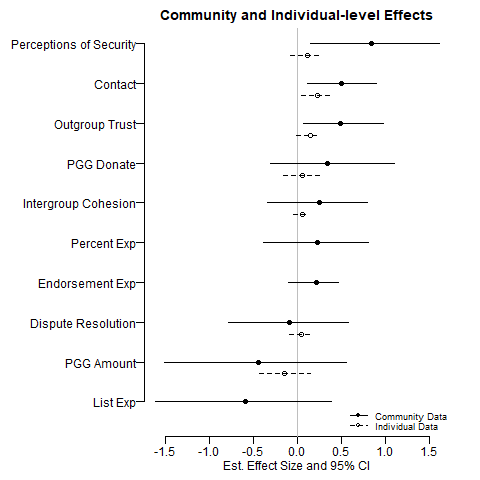
\includegraphics{../../../../figs/ecpn_coefplots_indices.png}

\hypertarget{small-number-of-communities}{%
\subsubsection{Small Number of
Communities}\label{small-number-of-communities}}

The main limitation of the community-level randomized controlled trial
is the number of communities we were able to include in the study. With
30 communities clustered at 15 sites, we have relatively low power to
detect an effect of ECPN. We try to increase power by testing multiple
hypotheses simultaneously (following Caughey, Dafoe, and Seawright 2017)
and by using inverse-covariance-weighted outcome indices, which should
measure our outcomes of interest more precisely than indices constructed
using other methods.

\hypertarget{self-selection-at-the-individual-level}{%
\subsubsection{Self-Selection at the Individual
Level}\label{self-selection-at-the-individual-level}}

We also initially planned to randomize participation on ECPN committees
within intervention communities. However, as discussed above, we had low
compliance with the individual-level randomization. As a result, many of
the people on the committees self-selected into participation. If we see
positive change among committee participants, therefore, it is possible
that the type of people who participated would have changed more
positively even without ECPN, making it difficult to attribute the
change to ECPN. It is also possible that ECPN is effective only on the
type of people who elected to participate and would not be as effective
on people less interested in the program, making it difficult to
generalize the effects of ECPN to the wider population in these areas.

We try to address these concerns in three ways. First, we illustrate
that the respondents we resurveyed are not statistically different from
baseline respondents on baseline measures. Since the people we
resurveyed are an as-if-random sample of all baseline respondents,
effects we see in this sample should generalize to other respondents.
Second, we demonstrate that on most measures, there are no measurable
baseline differences between direct participants, indirect participants,
and controls. When there are differences, the control sites start out
more positively than intervention sites, which would make it more
difficult for us to see an effect (i.e., the differences work against
us). Third, we present evidence that these groups do not differ in their
baseline-to-endline changes on two placebo outcomes, suggesting that
they have similar trajectories in the absence of ECPN. The results of
these balance and placebo tests are presented in Appendix 4.

\hypertarget{displacement}{%
\subsubsection{Displacement}\label{displacement}}

additional limitation of both analyses was the significant displacement
in Benue state at the time of the endline. Widespread violence between
farmers and pastoralists had forced many of the communities in Benue to
flee to safer locations. While we chose randomly among the people we
could find, we do not know whether the community members we could locate
were somehow different from the broader population in these communities.
Appendix 1 presents evidence that on measured variables, resurveyed
respondents in the individual-level analysis are representative of all
people from the baseline; we are not able to conduct a similar analysis
with the community-level sample. In the discussion section, we provide
further explanations for how the interpretation of our results would
change if our sample is unrepresentative due to displacement.

\hypertarget{program-adaptations}{%
\subsubsection{Program Adaptations}\label{program-adaptations}}

Finally, due to the fluid nature of conflict dynamics and the need to
adapt the program when necessary, we were not able to maintain
separation between intervention and control sites (i.e., there was
contamination). For example, the team conducted an intercommunity peace
forum in one intervention site, but community leaders requested that
leaders from a neighboring site---which happened to be a control
site---attend the forum because of a recent conflict event that had
spread across the area. The program team decided to risk contamination
of the research by including the control site in that one forum, for the
sake of the program's success. This type of contamination was limited as
much as possible, and to the extent that it may affect results of the
study, it would attenuate the results, working against our hypotheses
rather than in favor of them.

\hypertarget{discussion}{%
\section{Discussion}\label{discussion}}

Take-away: Evidence that this peacebuilding intervention increased trust
between conflicting groups. And group members feelings of physical
security increased.

More work to confirm effect, specify conditions and mechanisms. Not
clear that program improved attitudes/reduced animosity, other than
trust and social distance. No significant increase in cohesion. No
reduction in threat.

Not clear that the program increased people's confidence in dispute
resolution systems.

Mechanism could be ``ability to identify local outgroup from non-local
outgroup''?

Farmers arresting livestock guard suggests some level of ingroup
policing or of viewing the farmer and pastoralist communities as tied
together.

Bridging formal theory and rationalist perspectives with psychological
perspectives. Thinking about psychological implications on games like
bargaining, prisoner's dilemma/collective action problems, stag hunt,
and trust/trust + reassurance games. How do psychological conditions
like prejudice change preferences and behavior in these games? Ostrom
called for interdisciplinary work about variables affecting likelihood
of collective action (Ostrom and Walker 2003). Cannot always test these
variables in a lab -- groups have histories that create trut and
distrust, violence occurs in real world, signals of trust are embedded
in and can get dwarfed by wider social contexts, my self-conception as a
``nice'' person is connected to my real world behavior but maybe not my
lab behavior, etc\ldots{}

Farmer-pastoralist situation is like an infinitely repeating game. Gives
each group the incentive to cooperate so that the other side will
cooperate in the future.

We see more market interactions. Rohner, Thoenig, and Zilibotti (2013)
says trade can increase intergroup trust. More opportunities to signal
trustworthiness in trade. More opportunities to see benefit from
cooperating with the outgroup (Realistic group conflict theory).

Valuable to think bottom-up and top-down together. Some calls for more
attention to bottom-up approaches (Autesserre 2016, 2017; Ditlmann,
Samii, and Zeitzoff 2017; Safunu 2012).

Would this happen without NGO? Presence of outside group encouraging the
interaction surely helps. But the situations that these programs
exogenously introduce are often mimicked and inspired by real-life
experiences of villages that did not descend into conflict. Notable
in\ldots{}{[}chris: I think cites are all in autesserre2017 foreign
affairs. Stuff about Congo? Resisting War: How Communities Protect
Themselves. {]}. This program ``randomly assigns'' what those villages
developed endogenously.

Cannot \emph{only} be bottom-up. Context and policy matter, and elites
and governments control policy and set the context.

Future: mechanisms and ways to scale up. Mechanisms could be many
things. Ways to scale up: cannot have every group in conflict meet.
Scale up with contact between key actors that could diffuse the positive
effects of contact \& change social norms. Media programs and
observational/vicarious contact.

Some mechanisms of intergrop contact theory clearly will not function
here. Reduced outgroup threat ((``Sullivan, Pierson, \& Marcus, 1982;
Gibson, 2006). If citizens perceive or experience threat from an
out-group, they are more likely to be intolerant toward that group)''.
Ingroup expands to include outgroup -- no way. Empathy yes. Belief that
working together will benefit us == yes.

Other Mechanisms: assist intergroup bargaining with opportunities for
costly signaling, increased trust. Increase ingroup policing. Increase
social norms against intergroup violence. Change interpsonal attitudes?

An important question is scaling intergroup contact to larger conflicts.
Intergroup contact is unlikely to deter violence between groups involved
in large-scale ethnic war where opposing armies commit atrocities, for
example. It's also unlikely to naturally occur between groups with
limited contact to each other, or for people who consciously select out
of intergroup contact situations.

An attempt to scale-up intergroup contact can use mechanisms of social
or vicarious learning. Research shows that even \emph{observing}
interactions between a member of your group and a member of a disliked
group can improve attitudes (Vezzali et al. 2014). Television and radio
programs may thus provide intergroup contact between groups with limited
exposure to each other (Eller et al. 2011). ({\textbf{???}}) used
dramatic radio programs to influence attitudes and behaviors in a
post-conflict setting to some effect, and a similar strategy could be
used in a conflict setting. Future work should further investigate
mechanisms through which grassroots strategies can be successful.
Conditions under which different conflict resolution strategies are
successful -- when outside actors needed, when groups can be assisted in
solving own conflict. Future work should also investigate ``scaling up''
grassroots interventions, especially those involving intergroup contact.
Not every conflicting group can have contact with the other side.
Contact between key actors that could diffuse the positive effects of
contact \& change social norms. And research shows that even
\emph{observing} interactions between a member of your group and a
member of a disliked group can improve attitudes (Vezzali et al. 2014).
Television and radio programs may thus provide intergroup contact
between groups with limited exposure to each other (Eller et al. 2011).

Could be social desirability bias? Would indicate the program changed
social norms -- still valuable.

Could be survey acquescence bias -- randomization exp ``yes'' up on all
topics. But other ``placebo'' outcomes don't go up.

More research needed about using intergroup contact to promote peace
between people in conflict.

\hypertarget{references}{%
\section*{References}\label{references}}
\addcontentsline{toc}{section}{References}

\hypertarget{refs}{}
\leavevmode\hypertarget{ref-nyt2018nigeria}{}%
Akinwotu, Emmanuel. 2018. ``Nigeria's Farmers and Herders Fight a Deadly
Battle for Scarce Resources.'' \emph{New York Times}.
\url{https://www.nytimes.com/2018/06/25/world/africa/nigeria-herders-farmers.html}.

\leavevmode\hypertarget{ref-allison1985group}{}%
Allison, Scott T, and David M Messick. 1985. ``The Group Attribution
Error.'' \emph{Journal of Experimental Social Psychology} 21(6):
563--79.

\leavevmode\hypertarget{ref-allport1954prejudice}{}%
Allport, Gordon. 1954. ``The Nature of Prejudice.'' \emph{Garden City,
NJ Anchor}.

\leavevmode\hypertarget{ref-amir1969contact}{}%
Amir, Yehuda. 1969. ``Contact Hypothesis in Ethnic Relations.''
\emph{Psychological bulletin} 71(5): 319.

\leavevmode\hypertarget{ref-autesserre2016failure}{}%
Autesserre, Severine. 2016. ``The Responsibility to Protect in Congo:
The Failure of Grassroots Prevention.'' \emph{International
Peacekeeping} 23(1): 29--51.

\leavevmode\hypertarget{ref-autesserre2017international}{}%
---------. 2017. ``International Peacebuilding and Local Success:
Assumptions and Effectiveness.'' \emph{International Studies Review}
19(1): 114--32.

\leavevmode\hypertarget{ref-axelrod1980effective}{}%
Axelrod, Robert. 1980a. ``Effective Choice in the Prisoner's Dilemma.''
\emph{Journal of conflict resolution} 24(1): 3--25.

\leavevmode\hypertarget{ref-axelrod1980more}{}%
---------. 1980b. ``More Effective Choice in the Prisoner's Dilemma.''
\emph{Journal of Conflict Resolution} 24(3): 379--403.

\leavevmode\hypertarget{ref-bandura1999moral}{}%
Bandura, Albert. 1999. ``Moral Disengagement in the Perpetration of
Inhumanities.'' \emph{Personality and social psychology review} 3(3):
193--209.

\leavevmode\hypertarget{ref-barnhardt2009near}{}%
Barnhardt, Sharon. 2009. ``Near and Dear? Evaluating the Impact of
Neighbor Diversity on Inter-Religious Attitudes.'' \emph{Unpublished
working paper}.

\leavevmode\hypertarget{ref-beardsley2008agreement}{}%
Beardsley, Kyle. 2008. ``Agreement Without Peace? International
Mediation and Time Inconsistency Problems.'' \emph{American journal of
political science} 52(4): 723--40.

\leavevmode\hypertarget{ref-beber2012international}{}%
Beber, Bernd. 2012. ``International Mediation, Selection Effects, and
the Question of Bias.'' \emph{Conflict Management and Peace Science}
29(4): 397--424.

\leavevmode\hypertarget{ref-brewer1991social}{}%
Brewer, Marilynn B. 1991. ``The Social Self: On Being the Same and
Different at the Same Time.'' \emph{Personality and social psychology
bulletin} 17(5): 475--82.

\leavevmode\hypertarget{ref-brewer1999ingroupOutgroup}{}%
---------. 1999. ``The Psychology of Prejudice: Ingroup Love and
Outgroup Hate?'' \emph{Journal of social issues} 55(3): 429--44.

\leavevmode\hypertarget{ref-burns2015interaction}{}%
Burns, Justine, Lucia Corno, and Eliana La Ferrara. 2015.
\emph{Interaction, Prejudice and Performance. Evidence from South
Africa}. Working paper.

\leavevmode\hypertarget{ref-cotula2004land}{}%
Cotula, Lorenzo, Camilla Toulmin, Ced Hesse, and others. 2004.
\emph{Land Tenure and Administration in Africa: Lessons of Experience
and Emerging Issues}. International Institute for Environment;
Development London.

\leavevmode\hypertarget{ref-crescenzi2011supply}{}%
Crescenzi, Mark JC, Kelly M Kadera, Sara McLaughlin Mitchell, and
Clayton L Thyne. 2011. ``A Supply Side Theory of Mediation 1.''
\emph{International Studies Quarterly} 55(4): 1069--94.

\leavevmode\hypertarget{ref-daniel2018anti}{}%
Daniel, Soni. 2018. ``Anti-Open Grazing Law: Nass, Benue, Kwara, Taraba
Tackle Defence Minister.'' \emph{Vanguard}.
\url{https://www.vanguardngr.com/2018/06/anti-open-grazing-law-nass-benue-kwara-taraba-tackle-defence-minister/}.

\leavevmode\hypertarget{ref-di2017effectiveness}{}%
Di Salvatore, Jessica, and Andrea Ruggeri. 2017. ``Effectiveness of
Peacekeeping Operations.'' \emph{Oxford Research Encyclopedia of
Politics}.

\leavevmode\hypertarget{ref-ditlmann2016can}{}%
Ditlmann, Ruth K, and Cyrus Samii. 2016. ``Can Intergroup Contact Affect
Ingroup Dynamics? Insights from a Field Study with Jewish and
Arab-Palestinian Youth in Israel.'' \emph{Peace and Conflict: Journal of
Peace Psychology} 22(4): 380.

\leavevmode\hypertarget{ref-ditlmann2017addressing}{}%
Ditlmann, Ruth K, Cyrus Samii, and Thomas Zeitzoff. 2017. ``Addressing
Violent Intergroup Conflict from the Bottom up?'' \emph{Social Issues
and Policy Review} 11(1): 38--77.

\leavevmode\hypertarget{ref-doyle2000international}{}%
Doyle, Michael W, and Nicholas Sambanis. 2000. ``International
Peacebuilding: A Theoretical and Quantitative Analysis.'' \emph{American
political science review} 94(4): 779--801.

\leavevmode\hypertarget{ref-dreu2010social}{}%
Dreu, Carsten KW de. 2010. ``Social Value Orientation Moderates Ingroup
Love but Not Outgroup Hate in Competitive Intergroup Conflict.''
\emph{Group Processes \& Intergroup Relations} 13(6): 701--13.

\leavevmode\hypertarget{ref-duru2018court}{}%
Duru, Peter. 2018. ``Court Stops Inspector General from Proscribing
Benue Livestock Guard.'' \emph{Vanguard}.
\url{https://www.vanguardngr.com/2018/11/court-stops-ig-from-proscribing-benue-livestock-guards/}.

\leavevmode\hypertarget{ref-economist2019militias}{}%
Economist, The. 2019. ``Malicious Malitias: States in the Sahel Have
Unleashed Ethnic Gangs with Guns.'' \emph{The Economist}.
\url{https://www.economist.com/middle-east-and-africa/2019/05/04/states-in-the-sahel-have-unleashed-ethnic-gangs-with-guns}.

\leavevmode\hypertarget{ref-eidelson2003dangerous}{}%
Eidelson, Roy J, and Judy I Eidelson. 2003. ``Dangerous Ideas: Five
Beliefs That Propel Groups Toward Conflict.'' \emph{American
Psychologist} 58(3): 182.

\leavevmode\hypertarget{ref-mazziotta2011vicarious}{}%
Eller, Anja et al. 2011. ``Vicarious Intergroup Contact Effects:
Applying Social-Cognitive Theory to Intergroup Contact Research.''
\emph{Group Processes \& Intergroup Relations} 14(2): 255--74.

\leavevmode\hypertarget{ref-enos2014causal}{}%
Enos, Ryan D. 2014. ``Causal Effect of Intergroup Contact on
Exclusionary Attitudes.'' \emph{Proceedings of the National Academy of
Sciences} 111(10): 3699--3704.

\leavevmode\hypertarget{ref-fearon1994domestic}{}%
Fearon, James D. 1994a. ``Domestic Political Audiences and the
Escalation of International Disputes.'' \emph{American political science
review} 88(3): 577--92.

\leavevmode\hypertarget{ref-fearon1994ethnic}{}%
---------. 1994b. ``Ethnic War as a Commitment Problem.'' In
\emph{Annual Meetings of the American Political Science Association},
2--5.

\leavevmode\hypertarget{ref-fearon1995rationalist}{}%
---------. 1995. ``Rationalist Explanations for War.''
\emph{International organization} 49(3): 379--414.

\leavevmode\hypertarget{ref-fearon1998commitment}{}%
---------. 1998. ``Commitment Problems and the Spread of Ethnic
Conflict.'' \emph{The international spread of ethnic conflict} 107.

\leavevmode\hypertarget{ref-fearon2004civil}{}%
---------. 2004. ``Why Do Some Civil Wars Last so Much Longer Than
Others?'' \emph{Journal of peace research} 41(3): 275--301.

\leavevmode\hypertarget{ref-fearon1996explaining}{}%
Fearon, James D, and David D Laitin. 1996. ``Explaining Interethnic
Cooperation.'' \emph{American political science review} 90(4): 715--35.

\leavevmode\hypertarget{ref-festinger1962cognitiveDissonance}{}%
Festinger, Leon. 1962. 2 \emph{A Theory of Cognitive Dissonance}.
Stanford university press.

\leavevmode\hypertarget{ref-fey2010shuttle}{}%
Fey, Mark, and Kristopher W Ramsay. 2010. ``When Is Shuttle Diplomacy
Worth the Commute? Information Sharing Through Mediation.'' \emph{World
Politics} 62(4): 529--60.

\leavevmode\hypertarget{ref-finseraas2017does}{}%
Finseraas, Henning, and Andreas Kotsadam. 2017. ``Does Personal Contact
with Ethnic Minorities Affect Anti-Immigrant Sentiments? Evidence from a
Field Experiment.'' \emph{European Journal of Political Research} 56(3):
703--22.

\leavevmode\hypertarget{ref-forbes1997ethnic}{}%
Forbes, Hugh Donald. 1997. \emph{Ethnic Conflict: Commerce, Culture, and
the Contact Hypothesis}. Yale University Press.

\leavevmode\hypertarget{ref-gaertner2014reducing}{}%
Gaertner, Samuel L, and John F Dovidio. 2014. \emph{Reducing Intergroup
Bias: The Common Ingroup Identity Model}. Psychology Press.

\leavevmode\hypertarget{ref-gaertner2000reducing}{}%
Gaertner, Samuel L et al. 2000. ``Reducing Intergroup Conflict: From
Superordinate Goals to Decategorization, Recategorization, and Mutual
Differentiation.'' \emph{Group Dynamics: Theory, Research, and Practice}
4(1): 98.

\leavevmode\hypertarget{ref-gubler2013humanizing}{}%
Gubler, Joshua R. 2013. ``When Humanizing the Enemy Fails: The Role of
Dissonance and Justification in Intergroup Conflict.'' In \emph{Annual
Meeting of the American Political Science Association},

\leavevmode\hypertarget{ref-gutsell2010empathy}{}%
Gutsell, Jennifer N, and Michael Inzlicht. 2010. ``Empathy Constrained:
Prejudice Predicts Reduced Mental Simulation of Actions During
Observation of Outgroups.'' \emph{Journal of experimental social
psychology} 46(5): 841--45.

\leavevmode\hypertarget{ref-frontera2018nigeria}{}%
Hailemariam, Adium. 2018. ``Nigeria: Violence in the Middle Belt Becomes
Major Concern for President Buhari.'' \emph{Frontera}.
\url{https://frontera.net/news/africa/nigeria-violence-in-the-middle-belt-becomes-major-concern-for-president-buhari/}.

\leavevmode\hypertarget{ref-council2019nigeria}{}%
Harwood, Asch. 2019. ``Update: The Numbers Behind Sectarian Violence in
Nigeria.'' \emph{Council on Foreign Relations}.
\url{https://www.cfr.org/blog/update-numbers-behind-sectarian-violence-nigeria}.

\leavevmode\hypertarget{ref-haslam2014dehumanization}{}%
Haslam, Nick, and Steve Loughnan. 2014. ``Dehumanization and
Infrahumanization.'' \emph{Annual review of psychology} 65: 399--423.

\leavevmode\hypertarget{ref-hewstone1990ultimate}{}%
Hewstone, Miles. 1990. ``The `Ultimate Attribution Error'? A Review of
the Literature on Intergroup Causal Attribution.'' \emph{European
Journal of Social Psychology} 20(4): 311--35.

\leavevmode\hypertarget{ref-hewstone2006intergroup}{}%
Hewstone, Miles et al. 2006. ``Intergroup Contact, Forgiveness, and
Experience of `the Troubles' in Northern Ireland.'' \emph{Journal of
Social Issues} 62(1): 99--120.

\leavevmode\hypertarget{ref-hoffmann2004role}{}%
Hoffmann, Irene, and Isiaka Mohammed. 2004. ``THE Role of Nomadic Camels
for Manuring Farmers'FIELDS in the Sokoto Close Settled Zone, Northwest
Nigeria.'' \emph{Nomadic Peoples} 8(1): 99--112.

\leavevmode\hypertarget{ref-hunter1991intergroup}{}%
Hunter, John A, Maurice Stringer, and RP Watson. 1991. ``Intergroup
Violence and Intergroup Attributions.'' \emph{British Journal of Social
Psychology} 30(3): 261--66.

\leavevmode\hypertarget{ref-klein1992motivated}{}%
Klein, William M, and Ziva Kunda. 1992. ``Motivated Person Perception:
Constructing Justifications for Desired Beliefs.'' \emph{Journal of
experimental social psychology} 28(2): 145--68.

\leavevmode\hypertarget{ref-kuusaana2015land}{}%
Kuusaana, Elias Danyi, and Kaderi Noagah Bukari. 2015. ``Land Conflicts
Between Smallholders and Fulani Pastoralists in Ghana: Evidence from the
Asante Akim North District (Aand).'' \emph{Journal of rural studies} 42:
52--62.

\leavevmode\hypertarget{ref-kydd2000trust}{}%
Kydd, Andrew. 2000. ``Trust, Reassurance, and Cooperation.''
\emph{International Organization} 54(2): 325--57.

\leavevmode\hypertarget{ref-kydd2003side}{}%
---------. 2003. ``Which Side Are You on? Bias, Credibility, and
Mediation.'' \emph{American Journal of Political Science} 47(4):
597--611.

\leavevmode\hypertarget{ref-kydd2006can}{}%
Kydd, Andrew H. 2006. ``When Can Mediators Build Trust?'' \emph{American
Political Science Review} 100(3): 449--62.

\leavevmode\hypertarget{ref-levine1972ethnocentrism}{}%
LeVine, Robert A, and Donald T Campbell. 1972. ``Ethnocentrism: Theories
of Conflict, Ethnic Attitudes, and Group Behavior.''

\leavevmode\hypertarget{ref-leyens2007infra}{}%
Leyens, Jacques-Philippe et al. 2007. ``Infra-Humanization: The Wall of
Group Differences.'' \emph{Social Issues and Policy Review} 1(1):
139--72.

\leavevmode\hypertarget{ref-lupia1998democratic}{}%
Lupia, Arthur, Mathew D McCubbins, and Lupia Arthur. 1998. \emph{The
Democratic Dilemma: Can Citizens Learn What They Need to Know?}
Cambridge University Press.

\leavevmode\hypertarget{ref-marmaros2006friendships}{}%
Marmaros, David, and Bruce Sacerdote. 2006. ``How Do Friendships Form?''
\emph{The Quarterly Journal of Economics} 121(1): 79--119.

\leavevmode\hypertarget{ref-mcdonnel2017graze}{}%
McDonnel, Tim. 2017. ``Why It's Now a Crime to Let Cattle Graze Freely
in 2 Nigerian States.'' \emph{National Public Radio (NPR)}.
\url{https://www.npr.org/sections/goatsandsoda/2017/12/12/569913821/why-its-now-a-crime-to-let-cattle-graze-freely-in-2-nigerian-states}.

\leavevmode\hypertarget{ref-mcdougal2015effect}{}%
McDougal, Topher L et al. 2015. ``The Effect of Farmer-Pastoralist
Violence on Income: New Survey Evidence from Nigeria's Middle Belt
States.'' \emph{Economics of Peace and Security Journal} 10(1): 54--65.

\leavevmode\hypertarget{ref-nigeria2014freedom}{}%
Network, Nigeria Research. 2014. ``Indigeneity, Belonging, and Religious
Freedom in Nigeria: Citizens' Views from the Street.'' \emph{5. NRN
Policy Brief}.

\leavevmode\hypertarget{ref-opotow1990moral}{}%
Opotow, Susan. 1990. ``Moral Exclusion and Injustice: An Introduction.''
\emph{Journal of social issues} 46(1): 1--20.

\leavevmode\hypertarget{ref-ostrom2000collective}{}%
Ostrom, Elinor. 2000. ``Collective Action and the Evolution of Social
Norms.'' \emph{Journal of economic perspectives} 14(3): 137--58.

\leavevmode\hypertarget{ref-ostrom2003trust}{}%
Ostrom, Elinor, and James Walker. 2003. \emph{Trust and Reciprocity:
Interdisciplinary Lessons for Experimental Research}. Russell Sage
Foundation.

\leavevmode\hypertarget{ref-ott1972mediation}{}%
Ott, Marvin C. 1972. ``Mediation as a Method of Conflict Resolution: Two
Cases.'' \emph{International Organization} 26(4): 595--618.

\leavevmode\hypertarget{ref-page2008little}{}%
Page-Gould, Elizabeth, Rodolfo Mendoza-Denton, and Linda R Tropp. 2008.
``With a Little Help from My Cross-Group Friend: Reducing Anxiety in
Intergroup Contexts Through Cross-Group Friendship.'' \emph{Journal of
personality and social psychology} 95(5): 1080.

\leavevmode\hypertarget{ref-paluck2017contact}{}%
Paluck, Elizabeth Levy, Seth Green, and Donald P Green. 2017. ``The
Contact Hypothesis Revisited.''

\leavevmode\hypertarget{ref-paolini2010negative}{}%
Paolini, Stefania, Jake Harwood, and Mark Rubin. 2010. ``Negative
Intergroup Contact Makes Group Memberships Salient: Explaining Why
Intergroup Conflict Endures.'' \emph{Personality and Social Psychology
Bulletin} 36(12): 1723--38.

\leavevmode\hypertarget{ref-parker2013lessons}{}%
Parker, Michael T, and Ronnie Janoff-Bulman. 2013. ``Lessons from
Morality-Based Social Identity: The Power of Outgroup `Hate,' Not Just
Ingroup `Love'.'' \emph{Social Justice Research} 26(1): 81--96.

\leavevmode\hypertarget{ref-pettigrew1979ultimate}{}%
Pettigrew, Thomas F. 1979. ``The Ultimate Attribution Error: Extending
Allport's Cognitive Analysis of Prejudice.'' \emph{Personality and
social psychology bulletin} 5(4): 461--76.

\leavevmode\hypertarget{ref-pettigrew2006meta}{}%
Pettigrew, Thomas F, and Linda R Tropp. 2006. ``A Meta-Analytic Test of
Intergroup Contact Theory.'' \emph{Journal of personality and social
psychology} 90(5): 751.

\leavevmode\hypertarget{ref-pettigrew2008does}{}%
---------. 2008. ``How Does Intergroup Contact Reduce Prejudice?
Meta-Analytic Tests of Three Mediators.'' \emph{European Journal of
Social Psychology} 38(6): 922--34.

\leavevmode\hypertarget{ref-powell2006war}{}%
Powell, Robert. 2006. ``War as a Commitment Problem.''
\emph{International organization} 60(1): 169--203.

\leavevmode\hypertarget{ref-rauchhaus2006mediation}{}%
Rauchhaus, Robert W. 2006. ``Asymmetric Information, Mediation, and
Conflict Management.'' \emph{World Politics} 58(2): 207--41.

\leavevmode\hypertarget{ref-reed2016bargaining}{}%
Reed, William, David Clark, Timothy Nordstrom, and Daniel Siegel. 2016.
``Bargaining in the Shadow of a Commitment Problem.'' \emph{Research \&
Politics} 3(3): 2053168016666848.

\leavevmode\hypertarget{ref-rohner2013war}{}%
Rohner, Dominic, Mathias Thoenig, and Fabrizio Zilibotti. 2013. ``War
Signals: A Theory of Trade, Trust, and Conflict.'' \emph{Review of
Economic Studies} 80(3): 1114--47.

\leavevmode\hypertarget{ref-safunu2012grassroots}{}%
Safunu, Banchani John-Paul. 2012. ``Do Grassroots Approaches and
Mobilization for Development Contribute to Post-Conflict Peacebuilding?
The Experience of Northern Ghana.'' \emph{Nairobi: Africa Leadership
Center}.

\leavevmode\hypertarget{ref-savun2008information}{}%
Savun, Burcu. 2008. ``Information, Bias, and Mediation Success.''
\emph{International studies quarterly} 52(1): 25--47.

\leavevmode\hypertarget{ref-scacco2018nigeria}{}%
Scacco, Alexandra, and Shana S Warren. 2018. ``Can Social Contact Reduce
Prejudice and Discrimination? Evidence from a Field Experiment in
Nigeria.'' \emph{American Political Science Review} 112(3): 654--77.

\leavevmode\hypertarget{ref-sherif1958superordinate}{}%
Sherif, Muzafer. 1958. ``Superordinate Goals in the Reduction of
Intergroup Conflict.'' \emph{American journal of Sociology} 63(4):
349--56.

\leavevmode\hypertarget{ref-smith2003mediation}{}%
Smith, Alastair, and Allan Stam. 2003. ``Mediation and Peacekeeping in a
Random Walk Model of Civil and Interstate War.'' \emph{International
Studies Review} 5(4): 115--35.

\leavevmode\hypertarget{ref-svensson2009brings}{}%
Svensson, Isak. 2009. ``Who Brings Which Peace? Neutral Versus Biased
Mediation and Institutional Peace Arrangements in Civil Wars.''
\emph{Journal of conflict resolution} 53(3): 446--69.

\leavevmode\hypertarget{ref-tajfel1981groups}{}%
Tajfel, Henri. 1981. \emph{Human Groups and Social Categories: Studies
in Social Psychology}. CUP Archive.

\leavevmode\hypertarget{ref-tam2007impact}{}%
Tam, Tania et al. 2007. ``The Impact of Intergroup Emotions on
Forgiveness in Northern Ireland.'' \emph{Group Processes \& Intergroup
Relations} 10(1): 119--36.

\leavevmode\hypertarget{ref-thomas2018sahara}{}%
Thomas, Natalie, and Sumant Nigam. 2018. ``Twentieth-Century Climate
Change over Africa: Seasonal Hydroclimate Trends and Sahara Desert
Expansion.'' \emph{Journal of Climate} 31(9): 3349--70.

\leavevmode\hypertarget{ref-unah2018nigeria}{}%
Unah, Linus. 2018. \emph{In Nigeria's Diverse Middle Belt, a Drying
Landscape Deepens Violent Divides}. Christian Science Monitor.

\leavevmode\hypertarget{ref-vezzali2014indirect}{}%
Vezzali, Loris et al. 2014. ``Improving Intergroup Relations with
Extended and Vicarious Forms of Indirect Contact.'' \emph{European
Review of Social Psychology} 25(1): 314--89.

\leavevmode\hypertarget{ref-walter2002committing}{}%
Walter, Barbara F. 2002. \emph{Committing to Peace: The Successful
Settlement of Civil Wars}. Princeton University Press.

\leavevmode\hypertarget{ref-weinstein2005autonomous}{}%
Weinstein, Jeremy M. 2005. ``Autonomous Recovery and International
Intervention in Comparative Perspective.'' \emph{Available at SSRN
1114117}.

\leavevmode\hypertarget{ref-weisel2015ingroup}{}%
Weisel, Ori, and Robert Böhm. 2015. ```Ingroup Love' and `Outgroup Hate'
in Intergroup Conflict Between Natural Groups.'' \emph{Journal of
experimental social psychology} 60: 110--20.

\leavevmode\hypertarget{ref-wood2000attitude}{}%
Wood, Wendy. 2000. ``Attitude Change: Persuasion and Social Influence.''
\emph{Annual review of psychology} 51(1): 539--70.

\leavevmode\hypertarget{ref-yablon2012we}{}%
Yablon, Yaacov B. 2012. ``Are We Preaching to the Converted? The Role of
Motivation in Understanding the Contribution of Intergroup Encounters.''
\emph{Journal of Peace Education} 9(3): 249--63.

\end{document}
